

\section{User Study}

To compare our solution with traditional setting, we provided three different types of communication manners to play Mute Robot. We divided users into two groups by whether they have the same native language or not. So there are common language and different language group respectively. Different language group are required to use their native language to communicate with each other. About our experiment, every team will have two players and be placed in two distinct rooms. Players play Mute Robot with each other through Internet connection. Totally we tested 24 groups with 48 users (34 male and 14 female), inclusive of 12 common language groups and 12 different language groups (36 Taiwanese, 5 Japanese, 2 German, 1 Netherlander,  1 Chilan,1 Iraqi,1 Russian,1 Guatemalan)。.

\subsection{Method}

In our experiment, we provided three different types of communication manners to play Mute Robot:
\begin{enumerate}
    \item Speaking: 
    traditional gameplay manner, user can communicate through speaking language.
    \item Body Language: 
    players can communicate through body language only.
    \item Both:
    Players can communicate with each other through speaking language and body language.
\end{enumerate}

In order to eliminate order effects, each user played Mute Robot with counterbalance by administering the various types of game in different sequence. After playing each type of Mute Robot, players will fill out an eSFQ\cite{eSFQ} questionnaire to evaluate gameplay experience. Besides, When players finished all three types of Mute Robot, they will need to fill out another final questionnaire and proceed user interview. It needs about 1 hour to finish our user study experiment. We would conduct video recording at all experiment process and used these video to do CPMs\cite{CPMs} (see Figure~\ref{fig:US1}), which used to evaluate user gameplay experience.

\begin{figure}[!h]
\centering
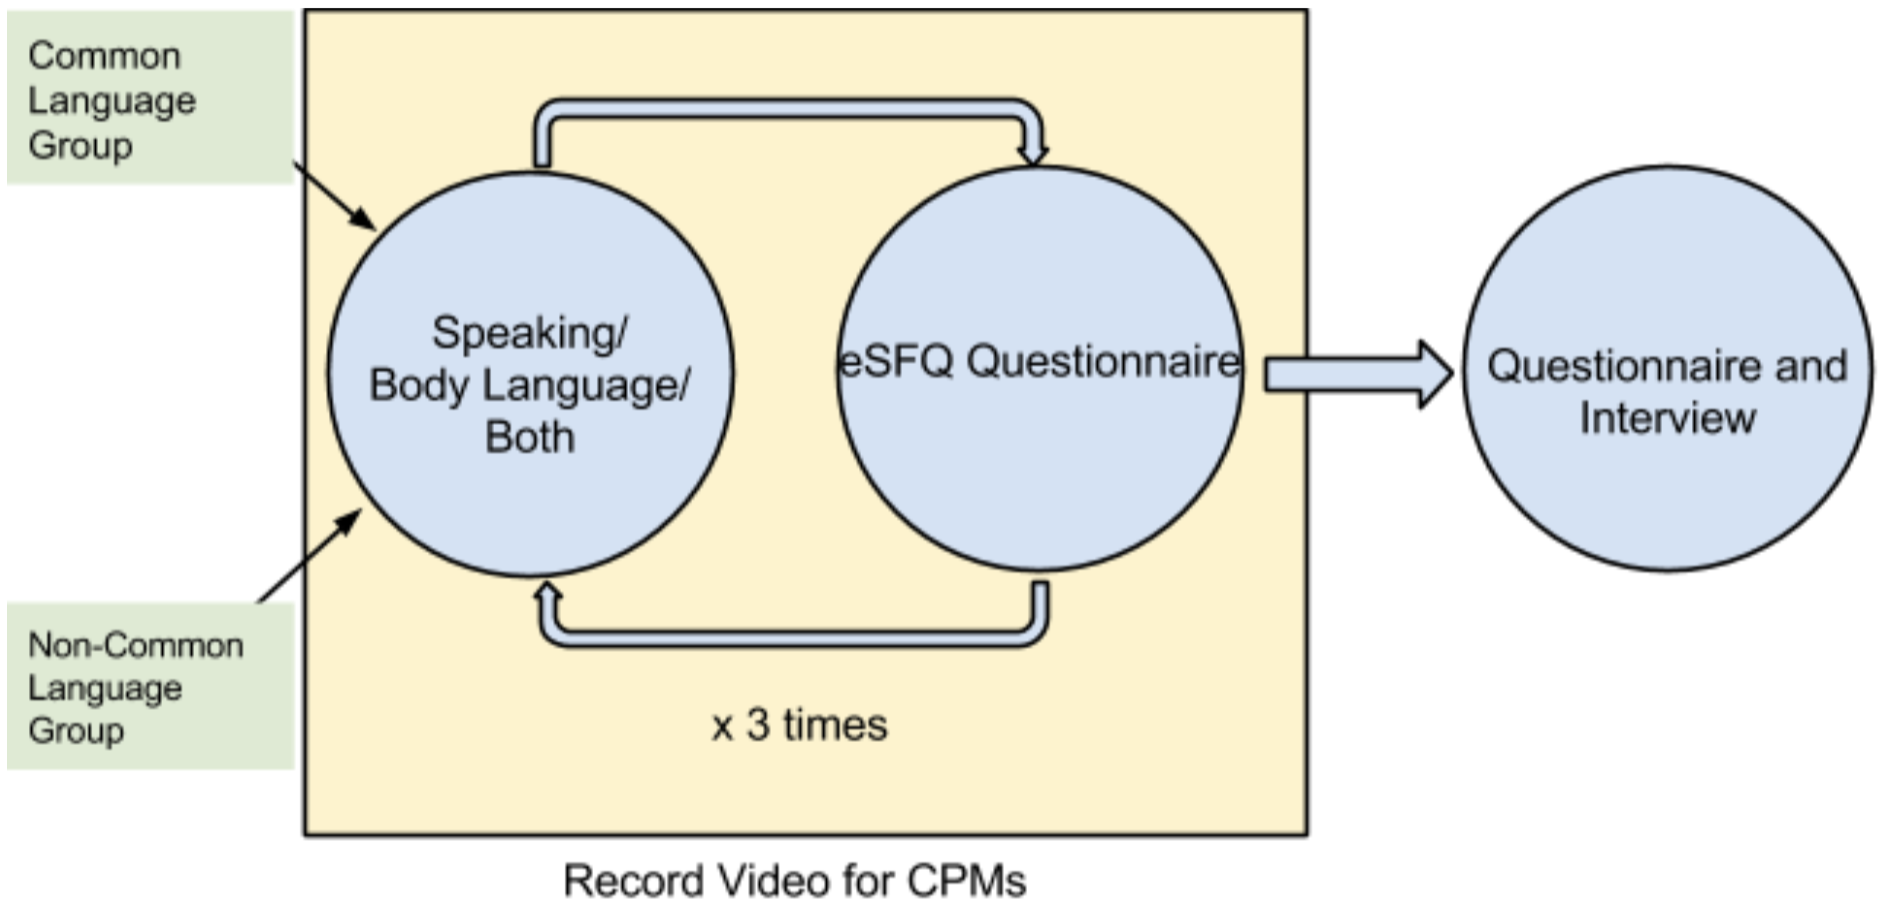
\includegraphics[width=0.9\columnwidth]{Figures/US_F1.png}
\caption{User study flow}
\label{fig:US1}
\end{figure}

\subsection{Result}
After our user study, we used eSFQ, CPMs, and Final questionnaire to evaluate the Mute Robot gameplay experience between different communication manners.

\subsubsection{eSFQ}
eSFQ\cite{eSFQ} had been proved that it is a questionnaire for rapid assessment of game experience. eSFQ capture the experienced fun/enjoyment, curiosity, and co-experience. 
% We used five-point likert scale ranging from ``I completely agree'', ``I agree'', ``neither/nor'', ``I disagree'' to ``I completely disagree''.

\paragraph{1. fun/enjoyment}

\begin{figure}[!h]
\centering
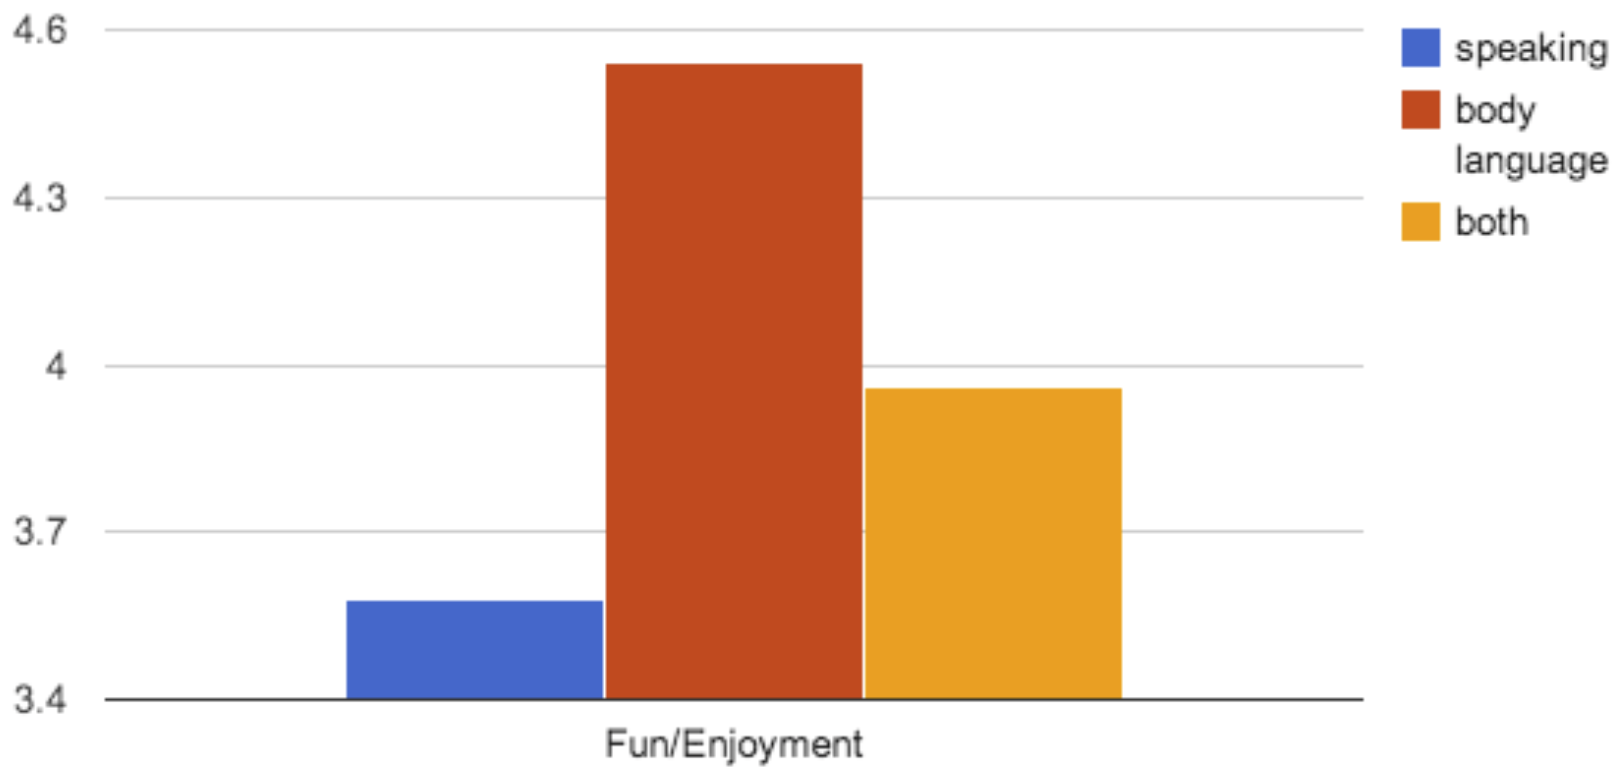
\includegraphics[width=0.9\columnwidth]{Figures/US_Fun_Com.png}
\caption{Common Language Group}
\label{fig:US_Fun_Com}
\end{figure}

\begin{figure}[!h]
\centering
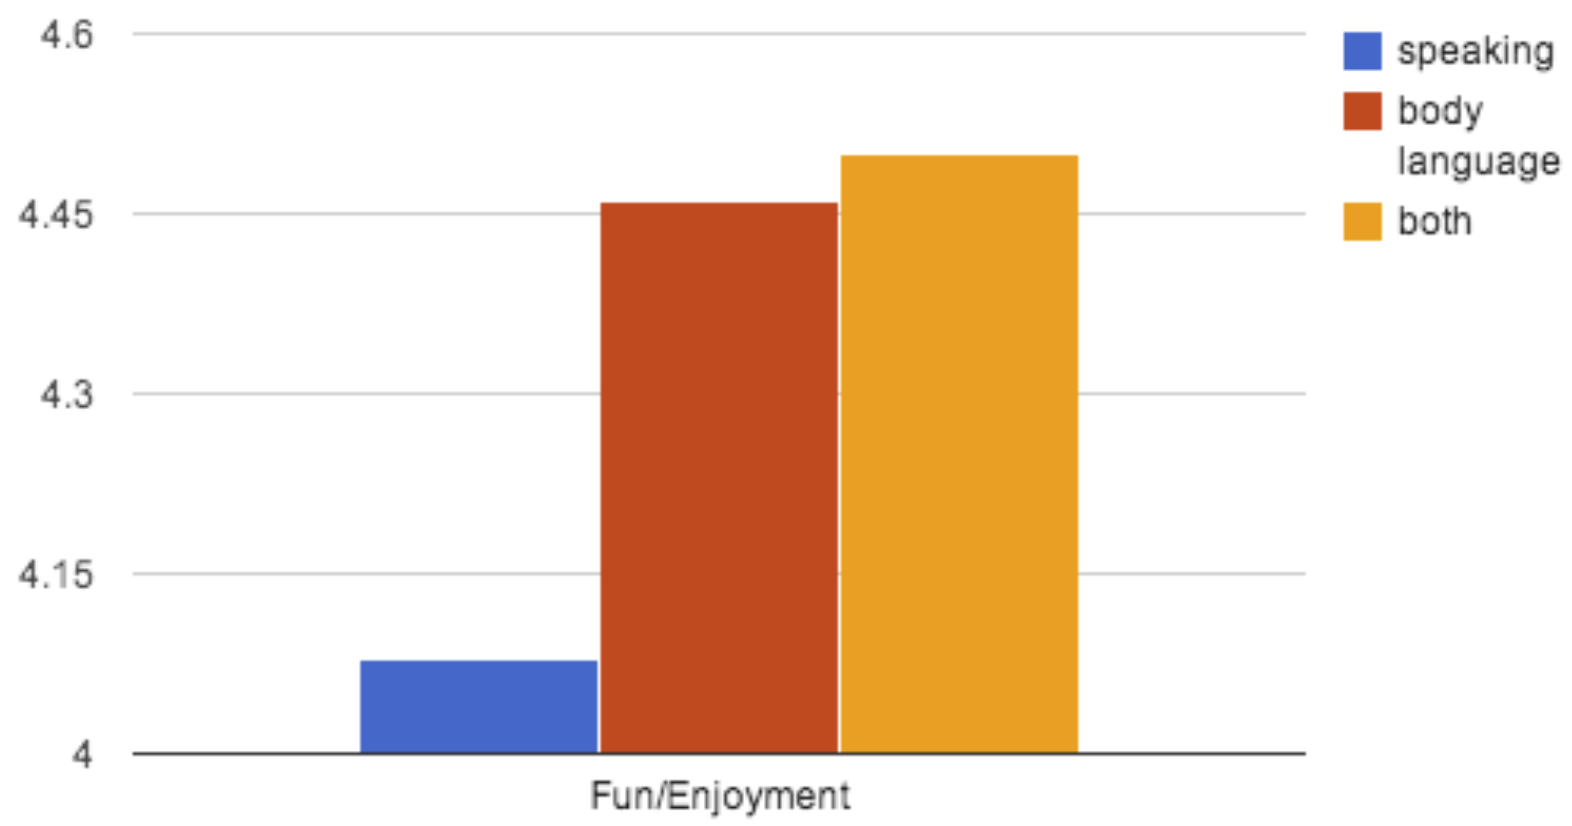
\includegraphics[width=0.9\columnwidth]{Figures/US_Fun_Dif.png}
\caption{Different Language Group}
\label{fig:US_Fun_Dif}
\end{figure}

\begin{figure}[!h]
\centering
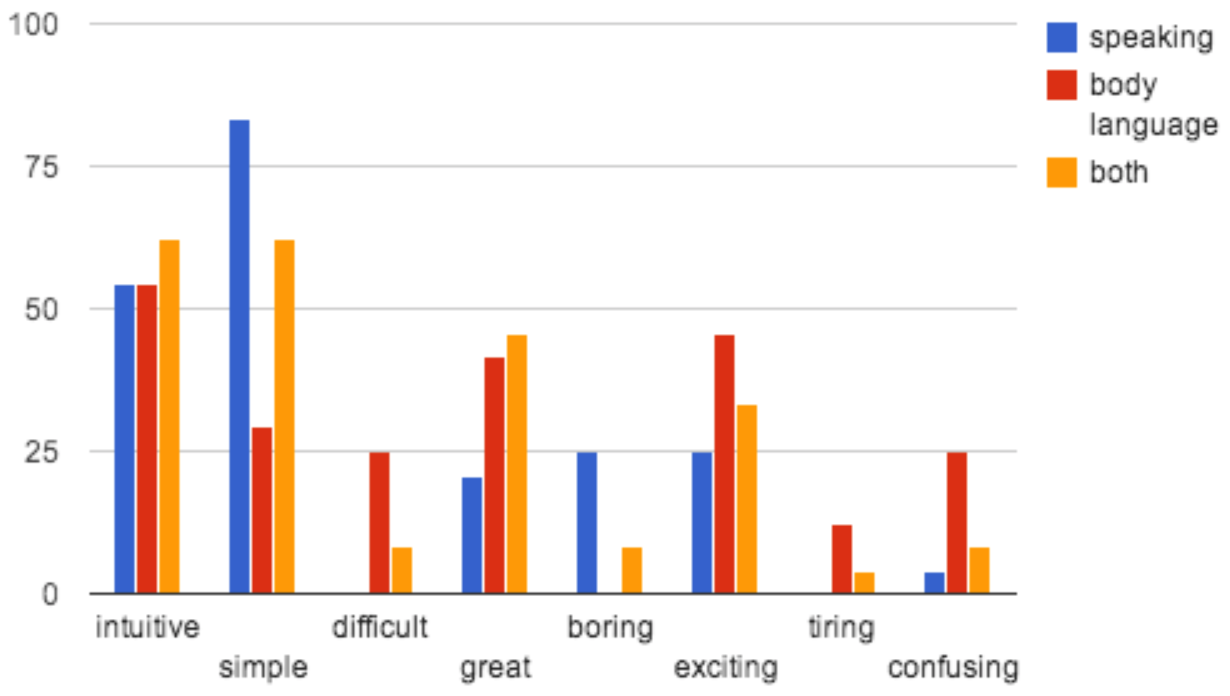
\includegraphics[width=0.9\columnwidth]{Figures/US_eSFQ_Com_Fun.png}
\caption{eSFQ: fun/enjoyment analysis for common language groups}
\label{fig:US_eSFQ_Com_Fun}
\end{figure}

\begin{figure}[!h]
\centering
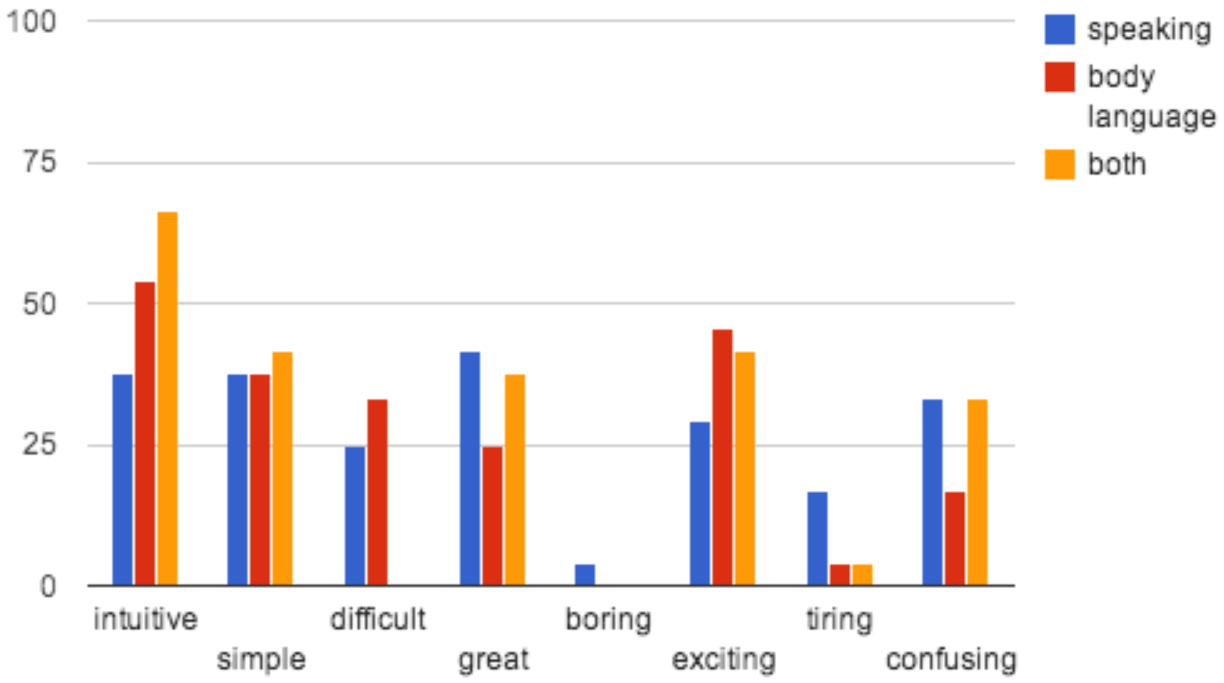
\includegraphics[width=0.9\columnwidth]{Figures/US_eSFQ_Dif_Fun.png}
\caption{eSFQ: fun/enjoyment analysis for different language groups}
\label{fig:US_eSFQ_Dif_Fun}
\end{figure}

For common language group (see Figure~\ref{fig:US_Fun_Com}), the mean of the experienced fun level for ``speaking'' was 3.58 (SD = 1.14) (5 meaning ``Yeah, fun'' - highest level of fun and 1 meaning ``Yawn, boring'' - lowest level of fun). Their game experiences were related to simple (83\% of the users), and intuitive(54\%). The mean of the experienced fun level for ``body language'' was 4.54 (SD = 0.66). Their game experiences were related to intuitive (54\%), exciting (46\%) and great (42\%). The mean of the experienced fun level for ``using speaking and body language together'' was 3.96 (SD = 1.00). Their game experiences were related to intuitive (63\%), simple (63\%) and exciting (33\%). 

For different language group (see Figure~\ref{fig:US_Fun_Dif}), the mean of the experienced fun level for ``speaking'' was 4.08 (SD = 0.97). Their game experiences were related to great (42\% of the users), intuitive (38\%), simple (38\%), and confusing (33\%). The mean of the experienced fun level for ``body language'' was 4.46 (SD = 0.66). Their game experiences were related to intuitive (54\%), exciting (46\%), simple (38\%) and difficult (33\%). The mean of the experienced fun level for ``using speaking and body language together'' was 4.50 (SD = 0.59). Their game experiences were related to intuitive (67\%), exciting (42\%), simple (42\%), great (34\%) and confusing (33\%).

% The fun/enjoyment rate of ``body language'' and ``using speaking and body language together'' were better than ``speaking'', no matter in common language group or in different language group. In sum, ``body language'' got the best rate of fun level, and the rate of ``using speaking and body language together'' was only slightly lower than ``body language'' but is still very good. And ``speaking'' got the worst rate. We dicovered that the difficulty of the game would make an influence on fun. In other words, both index were in direct proportion. For instance, when the ratio of simple becomes higher, the ratio of fun will be lower than before. In addition, different language group had higher experienced fun level for ``speaking'', but it also make users feeling confused for ``speaking'' and``using speaking and body language together''.

As we can see in Figure~\ref{fig:US_Fun_Com} and \ref{fig:US_Fun_Dif}, whether players have common language or not, body language has higher rate of fun/enjoyment than traditional manner(speaking). In other words, body language can enhance fun and enjoyment. According to Figure~\ref{fig:US_eSFQ_Com_Fun} and \ref{fig:US_eSFQ_Dif_Fun}, the confusing index was in contrast to common language group and different langauge group. Common language group felt that using body language was the most confused. However, different language group thought using body languagae was the least confused manner to communicate.

\paragraph{2. curiosity}

For common language group, the curiosity about ``speaking'' was rated with a mean of 4.01 (SD = 0.85 (5 meaning very curious and 1 meaning not curious at all). ``body language'' with 4.39 on average (SD = 0.74) and ``using speaking and body language together'' with 4.25 on average (SD = 0.73).

For different language group, the curiosity about ``speaking'' was rated with a mean of 4.04 (SD = 0.90). ``body language'' with 4.11 on average (SD = 0.93) and ``using speaking and body language together'' with 4.07 on average (SD = 0.89).

According to the curiousity index, we could find out that users were curious about the game. Analyzed data in detail, we could find out that ``body language'' had the highest rate. Second is ``using speaking and body language together'', and ``speaking'' has the worst rate. As a result, no matter in common language group or different language group, communication manners has no significant impact on the index of curiosity.

\begin{table}[!h]
\renewcommand\arraystretch{1.5}
  \centering
  \begin{tabular}{
  !{\vrule width2pt}c
  !{\vrule width2pt}c
  !{\vrule width2pt}c
  !{\vrule width2pt}c
  !{\vrule width2pt}}
    \Xhline{2pt}
    \multicolumn{1}
    {!{\vrule width2pt}c!{\vrule width2pt}}
    {\tabhead{}} &
    \multicolumn{1}
    {c!{\vrule width2pt}}
    {\centering\tabhead{Speaking}} &
    \multicolumn{1}
    {c!{\vrule width2pt}}
    {\centering\tabhead{Body Language}} &
    \multicolumn{1}
    {c!{\vrule width2pt}}
    {\centering\tabhead{Both}} \\
    \Xhline{2pt}
    Common Language & 4.01 & 4.39 & 4.25 \\
    \Xhline{2pt}
    Different Language & 4.04 & 4.11 & 4.07 \\
    \Xhline{2pt}
  \end{tabular}
  \caption{Curiosity index of eSFQ}
  \label{tab:KappaValue}
\end{table}


% we found out that in common language group, although the game is the same, curiosity still be impacted by communication manners. But different langauge group didn't have obvious difference.

% \begin{figure}[!h]
% \centering
% 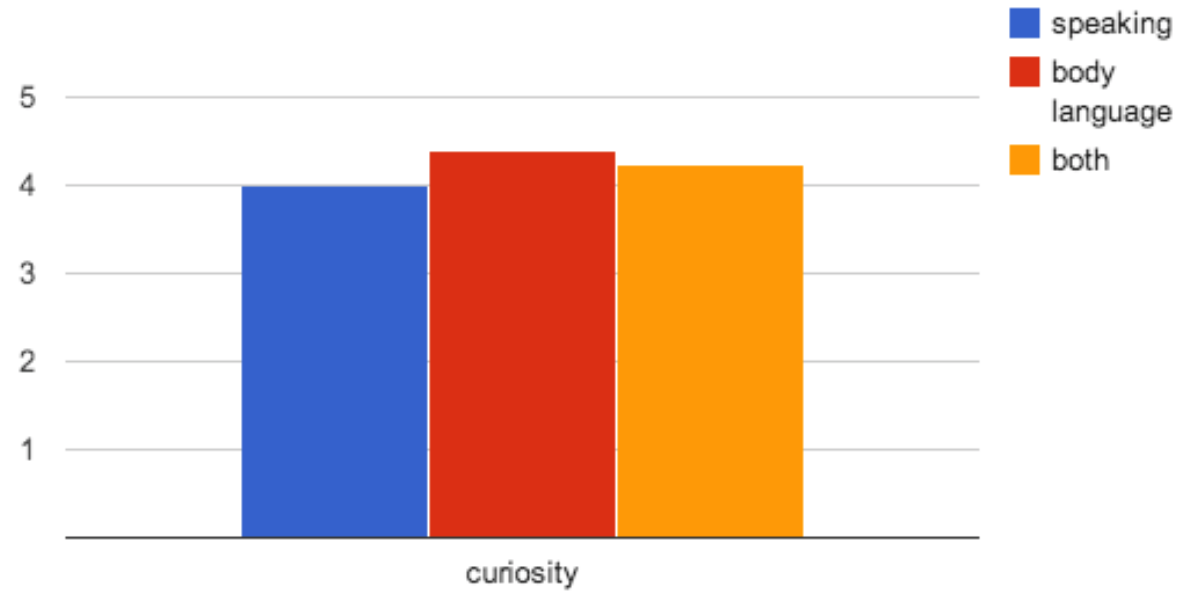
\includegraphics[width=0.9\columnwidth]{Figures/US_Curi_Com.png}
% \caption{Common Language Group}
% \label{fig:US_Curi_Com}
% \end{figure}

% \begin{figure}[!h]
% \centering
% 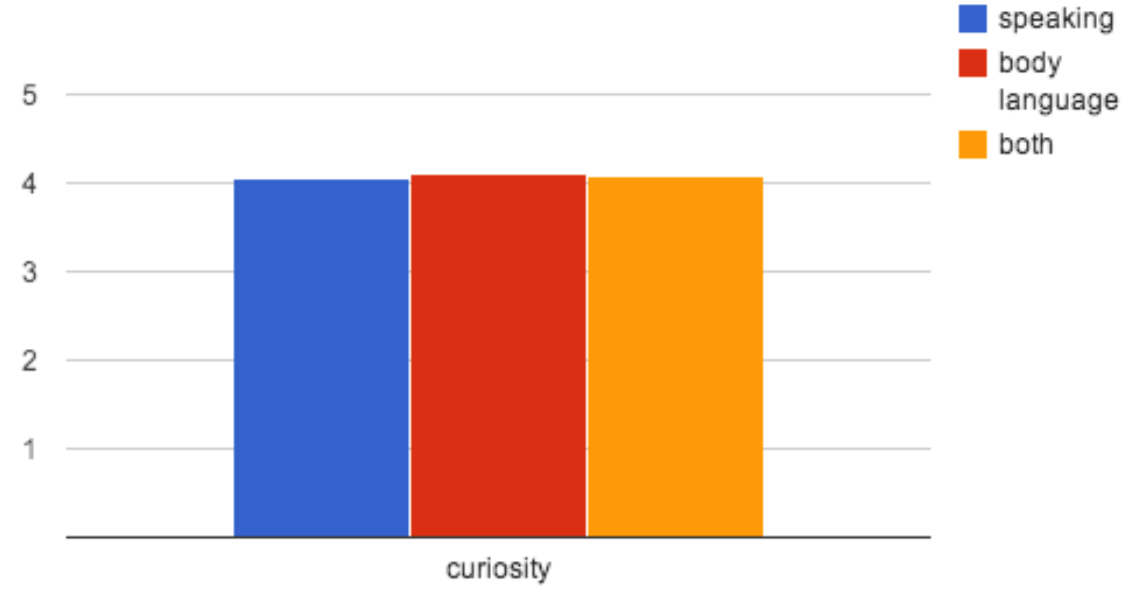
\includegraphics[width=0.9\columnwidth]{Figures/US_Curi_Dif.png}
% \caption{Different Language Group}
% \label{fig:US_Curi_Dif}
% \end{figure}


\paragraph{3. co-experience}

For common language group, the users experienced playing ``speaking'' together as cooperative (83\% of the users), fun (46\%) and happy (42\%). The users experienced playing ``body language'' together as cooperative (88\% of the user), fun (83\%), happy (50\%), encouraging (33\%) and satisfying (33\%). The users experienced playing ``using speaking and body language together'' together as cooperative (83\% of the user), fun (79\%), happy (67\%), satisfying (38\%) and triumphing (33\%).

For non-common language group,the users experienced playing ``speaking'' together as cooperative (83\% of the users), fun (54\%), happy (50\%) and frustrating (25\%). The users experienced playing ``body language'' together as cooperative (79\% of the user), fun (67\%), happy (58\%), satisfying (54\%) and frustrating (13\%). The users experienced playing ``using speaking and body language together'' together as cooperative (88\% of the user), fun (88\%), happy (58\%), satisfying (46\%) and frustrating (13\%). 

% The co-experience rate ``body language'' and ``using speaking and body langauge together'' were better than ``speaking'', no matter in common language group or in different language group. In different language group, ``speaking'' made 25\% people feel frustrated, and both ``body language'' and ``using speaking and body language togther'' are 13\%.

According to Figure~\ref{fig:US_Co-ex_Com_Pos}, ``body language'' communication manner has the highest fun index for common language group. In accordance with Figure~\ref{fig:US_Co-ex_Dif_Pos}, ``both'' communication manner has the highest fun index for different language group. However, from Figure~\ref{fig:US_Co-ex_Dif_Neg}, compared to traditional setting and body language setting, the frustrating rate decreases obviously from 25\% to 13\%, which means the ratio of frustrating decreased 48\%.


\begin{figure}[!h]
\centering
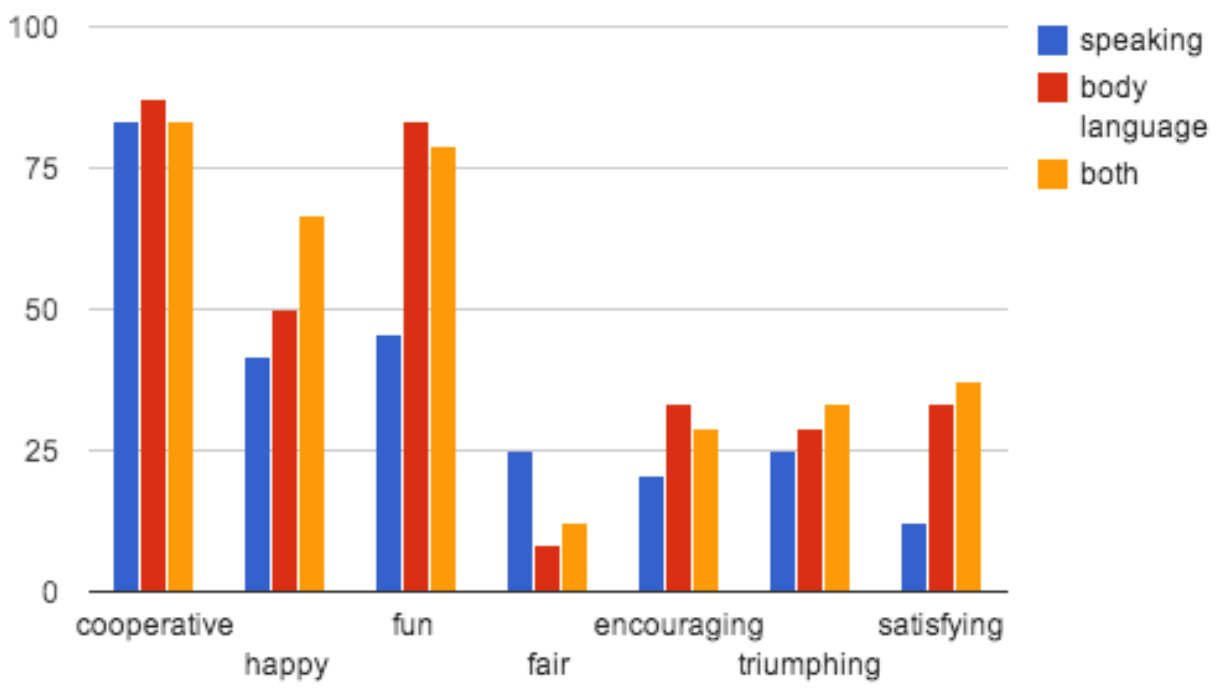
\includegraphics[width=0.9\columnwidth]{Figures/US_Co-ex_Com_Pos.png}
\caption{Positive Co-experience for Common Language Group}
\label{fig:US_Co-ex_Com_Pos}
\end{figure}

\begin{figure}[!h]
\centering
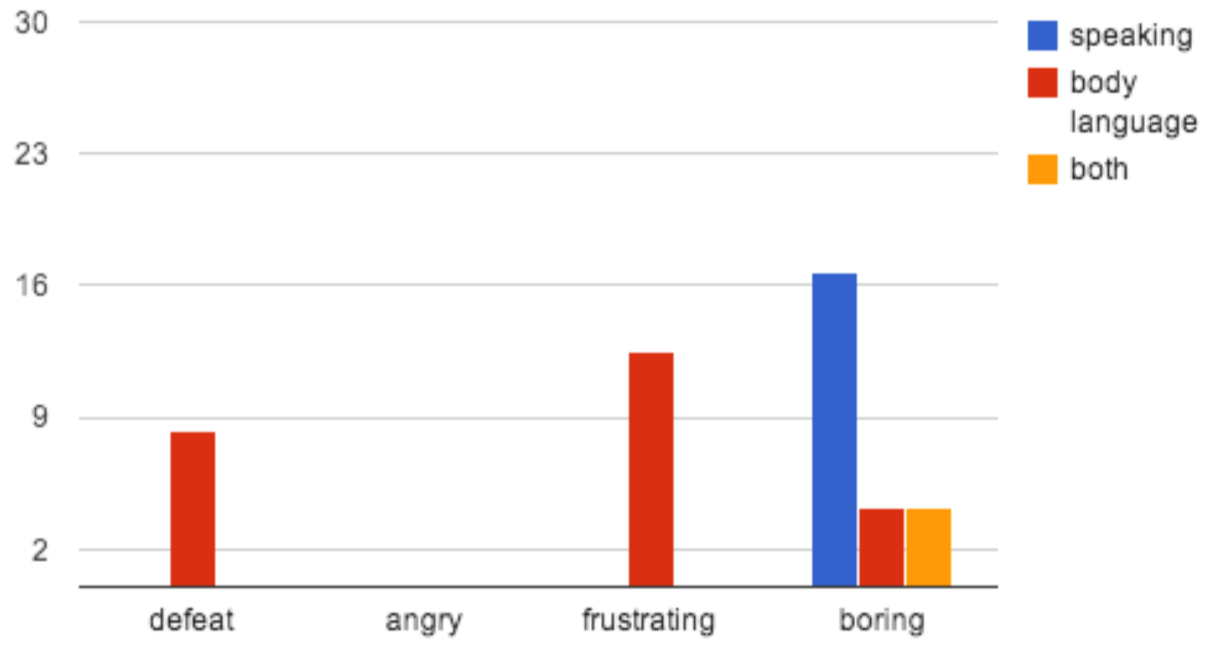
\includegraphics[width=0.9\columnwidth]{Figures/US_Co-ex_Com_Neg.png}
\caption{Negative Co-experience for Common Language Group}
\label{fig:US_Co-ex_Com_Neg}
\end{figure}

\begin{figure}[!h]
\centering
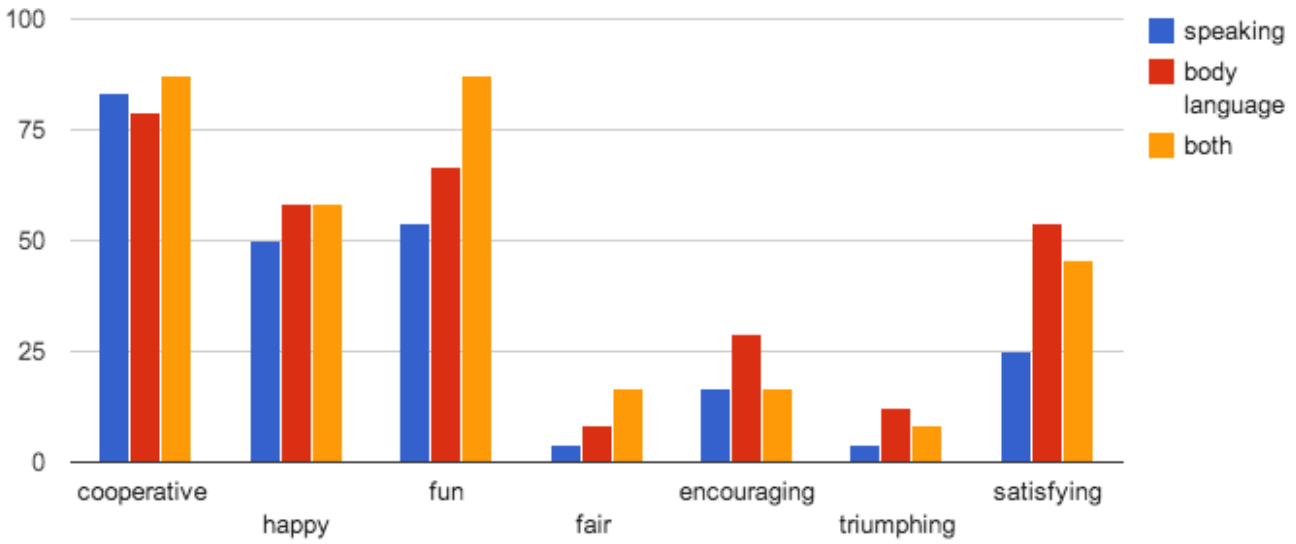
\includegraphics[width=0.9\columnwidth]{Figures/US_Co-ex_Dif_Pos.png}
\caption{Positive Co-experience for Different Language Group}
\label{fig:US_Co-ex_Dif_Pos}
\end{figure}

\begin{figure}[!h]
\centering
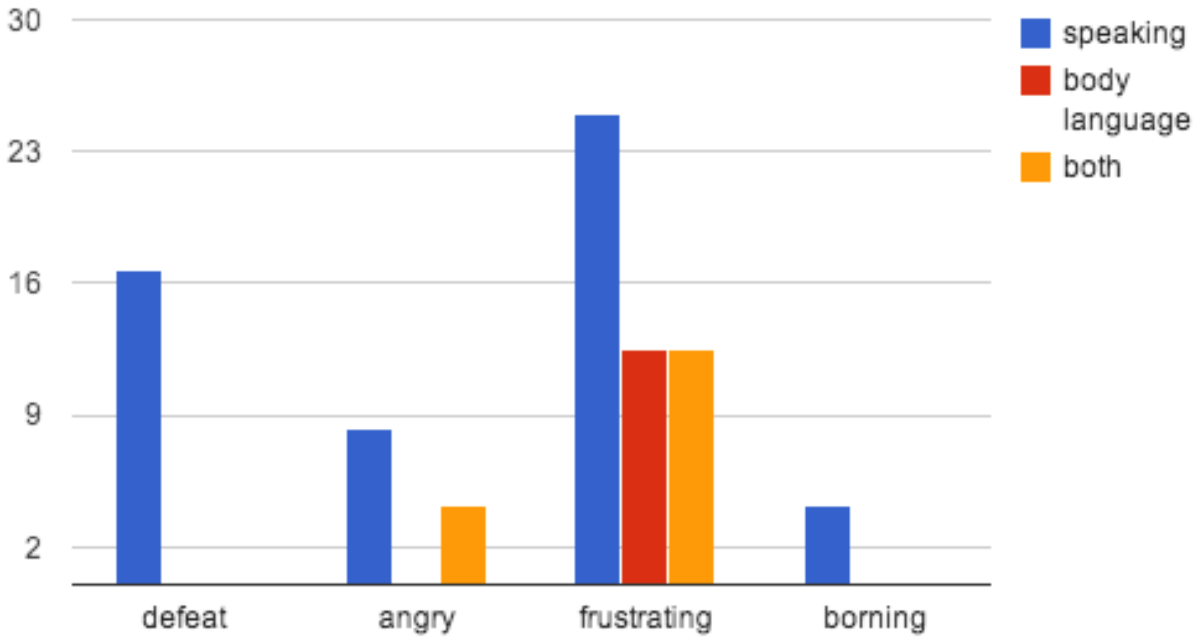
\includegraphics[width=0.9\columnwidth]{Figures/US_Co-ex_Dif_Neg.png}
\caption{Negative Co-experience for Different Language Group}
\label{fig:US_Co-ex_Dif_Neg}
\end{figure}


\subsubsection{CPMs}

Cooperative Performance Metrics (CPMs)\cite{CPMs} used for analysis of cooperative games. CPMs analyzed game experience manners through players' behavior during game playing. The set of CPMs developed is as follows: ``Laughter or excitement together'', ``Work out strategies'', ``Helping each other'', ``Global Strategies'', ``Waited for each other'' and ``Got in each other's way ''. 
% Because the index of ``Laugher or excitement together'' is unfair to body language communicatin manner, which can't hear another player's sound, thus we added an additinal index: ``Laugher or excitement'', which indicates count of personal user's laugh times, and 
After our user study, we found out that ``Global Strategies'' didn't happen in our game, and ``Got in each other's way'' only happened two times in our user study. So we removed these two indexes.

Futhermore, for each CPM label within the video analysis, the researcher identified a cause based on the cooperative design patterns. Thus, before discussing our results, we will discuss the validation process we performed to evaluate the reliability of the results. First, to establish face validity, patterns and CPMs were developed through an intensive review process. To establish scientific validity, we performed a formal validation process. We asked two independent researchers to rate four sessions given the CPMs and the cooperative patterns identified. All researchers read the CPMs in detail and were shown an example of how to apply them using a video-taped gameplay session. Afterwards, they were given four videos of play session to analyze. We then perform inter-rater agreement and calculated kappa values\cite{Kappa1,Kappa2}. 

Table~\ref{tab:KappaValue} shows the results of this process. Based on these results, the kappa value presented are sufficient to establish validity of the approach and the results.

\begin{table}[!h]
\renewcommand\arraystretch{1.5}
  \centering
  \begin{tabular}{
  !{\vrule width2pt}p{0.22\columnwidth}
  !{\vrule width2pt}p{0.08\columnwidth}
  !{\vrule width2pt}p{0.08\columnwidth}
  !{\vrule width2pt}p{0.08\columnwidth}
  !{\vrule width2pt}p{0.08\columnwidth}
  !{\vrule width2pt}p{0.08\columnwidth}
  !{\vrule width2pt}p{0.08\columnwidth}
  !{\vrule width2pt}}
    \Xhline{2pt}
    \multicolumn{1}
    {!{\vrule width2pt}c!{\vrule width2pt}}
    {\tabhead{\multirow{2}{*}{Inter-rater}}} &
    \multicolumn{6}
    {c!{\vrule width2pt}}
    {\centering\tabhead{Kappa for Metrics}} \\
    \Xcline{2-7}{2pt}
    % \hline
    & M1 & M2 & M3 & M4 & M5 & M6 \\
    \Xhline{2pt}
    Session1 & 0.75 & 1 & 0.79 & 1 & 1 & 1 \\
    \Xhline{2pt}
    Session2 & 1 & 0.8 & 1 & 1 & 1 & 1 \\
    \Xhline{2pt}
    Session3 & 0.75 & 1 & 0.87 & 1 & 1 & 1 \\
    \Xhline{2pt}
    Session4 & 1 & 1 & 0.96 & 1 & 1 & 1 \\
    \Xhline{2pt}
    Average & 0.88 & 1.2 & 0.91 & 1 & 1 & 1 \\
    \Xhline{2pt}
  \end{tabular}
  \caption{Inter-rater Agreement (M stands for CPM)}
  \label{tab:KappaValue}
\end{table}



For common language group (see Figure~\ref{fig:US_CPMs_Com}),
``body language'' communication cause more ``laughter or excitement'' and ``helping each other''.
For different language group (see Figure~\ref{fig:US_CPMs_Dif}), ``speaking'' and ``both'' communication manner cause more ``laughter or excitement''. We found that it is hard to trigger ``laugher or excitement'' without sound transmission. Compared to common language group and different langauge group, it shows that CPMs index of body language is similar, providing consistent experience.

 
% after the integration of our data, we could find out that ``body language'' occurred most frequently at CPMs indexes except index of ``Waited for each other''. Second is ``using speaking and body language together'', and ``speaking'' occurred least frequently. Furthermore, ``Helping each other'' and ``Laugher or excitement'' were in direct proportion. And ``Helping each other'' increased significantly while using body language communication manner.

% from the count of each index happened, we could conclude that ``using speaking and body language together'' had highest frequency to happen. Second is ``speaking'', and ``body language'' had lowest frequency to happen. In addition, making comparison between different language group and common language group, count of ``Helping each other'' of different language group increased significantly in ``speaking'' and ``using speaking and body language together'', and count of all CPMs indexes happened in ``body language'' were almost the same for common language group.


\begin{figure}[!h]
\centering
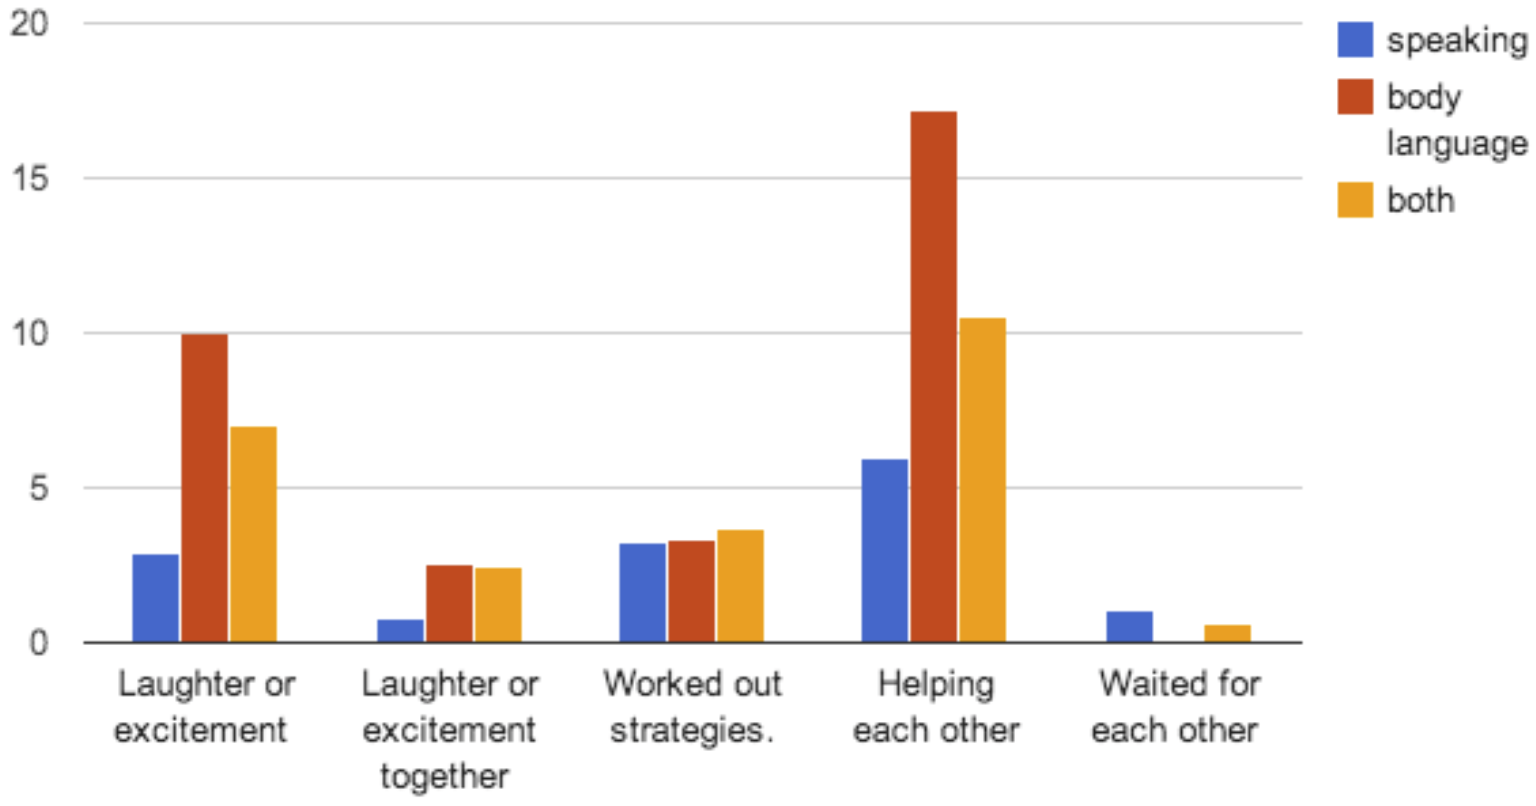
\includegraphics[width=0.9\columnwidth]{Figures/US_CPMs_Com.png}
\caption{Common Language Group}
\label{fig:US_CPMs_Com}
\end{figure}

\begin{figure}[!h]
\centering
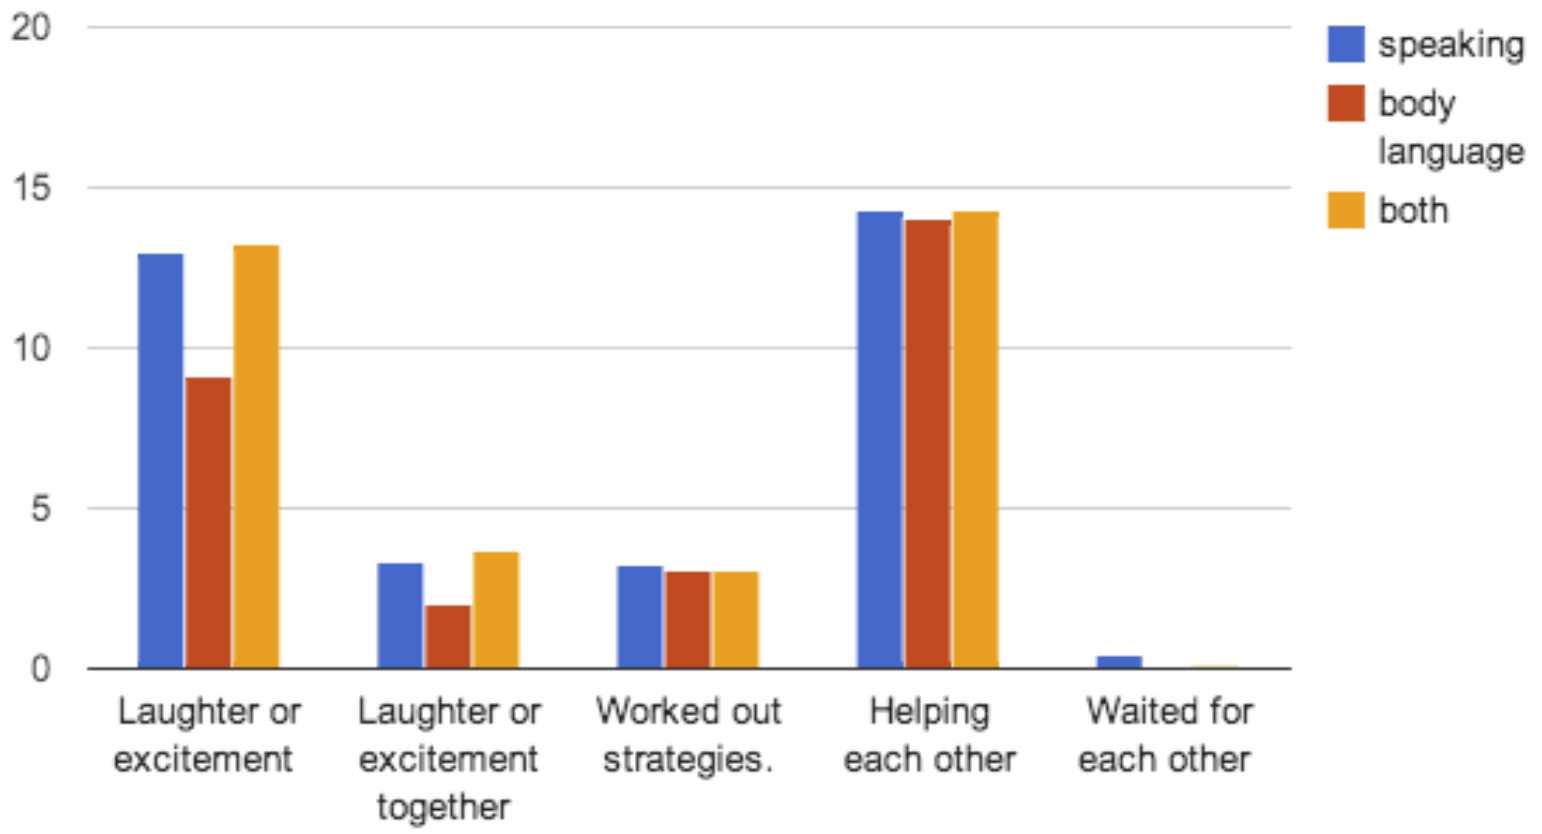
\includegraphics[width=0.9\columnwidth]{Figures/US_CPMs_Dif.png}
\caption{Different Language Group}
\label{fig:US_CPMs_Dif}
\end{figure}


\subsubsection{Final Questionnaire}
In order to thoroughly realize users' feedback, we designed an final questionnaire, which asked ``the most favorite'', ``the most interesting'', ``the easiest'', ``the most difficult'', ``the most intuitive'' and ``the best cooperative feeling's'' communication manners respectively with ``speaking'', ``body language'' and ``using speaking and body language together'' three distinct choice.

\paragraph{1. Common Language Group}
Our result presented on the diagram (see Figure~\ref{fig:US_FQ_Com}) for common language group. 
% We could find out that most users feel ``body language'' is the most difficult one. However, 
body language had the highest proportion in the index of ``favorite'', ``funniest'' and ``cooperative''.
% most people also felt ``body language'' is the most interesting, the best cooperative feeling's, and the most favorite communication manner. Another communication manner, ``using speaking and body language together'', also have good expression. From our statistics, users considered that ``using speaking and body language together'' has better gameplay interesting and cooperative feeling's than ``speaking''. 
And more than half of users felt ``speaking'' is the easiest, the most intuitive and the least interesting manner to communicate.

\begin{figure}[!h]
\centering
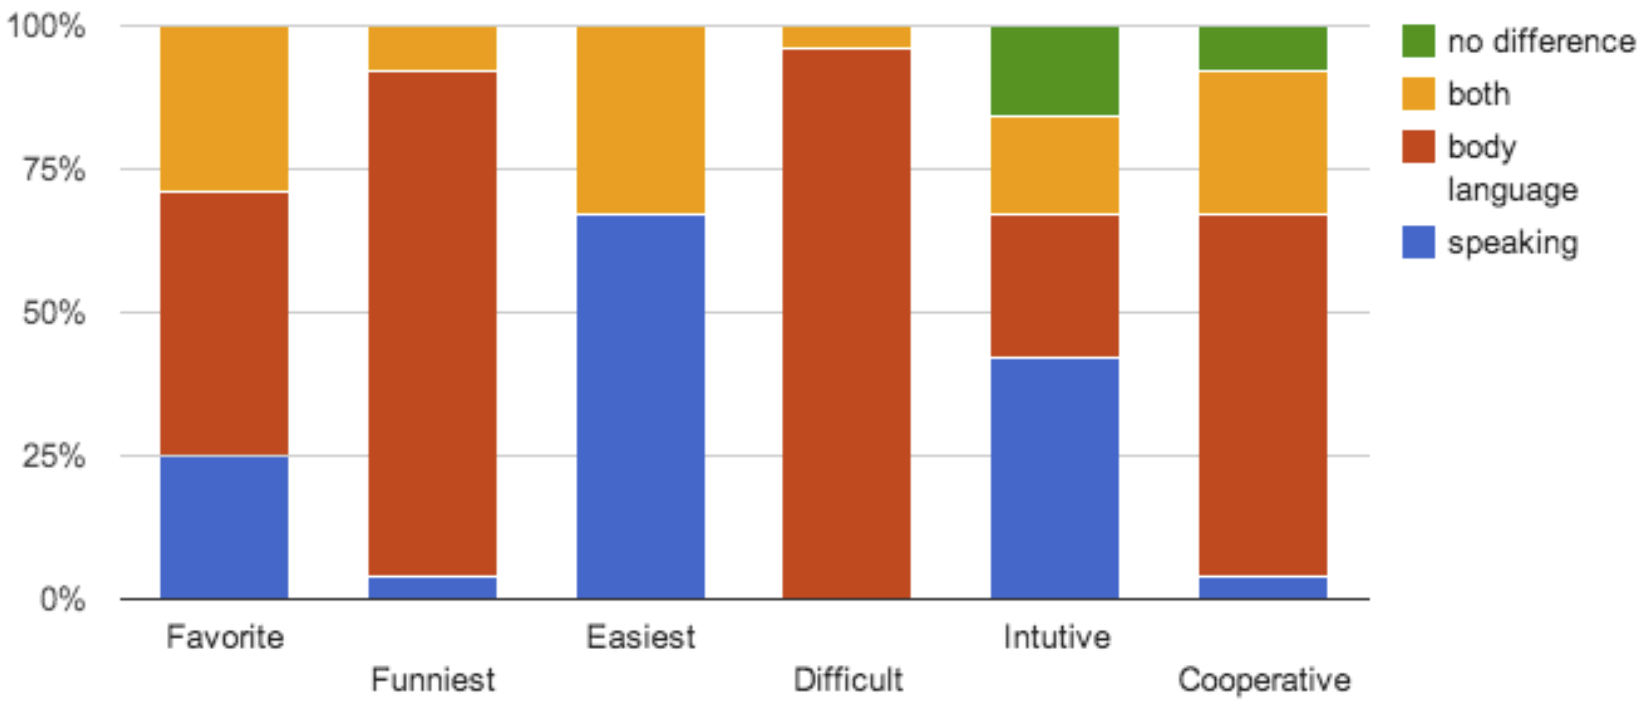
\includegraphics[width=0.9\columnwidth]{Figures/US_FQ_Com.png}
\caption{Common Language Group}
\label{fig:US_FQ_Com}
\end{figure}

\paragraph{2. Different Language Group}
From our statistic diagram (see Figure~\ref{fig:US_FQ_Dif}) for different langauge group, more than half of the users felt that ``speaking'' is the most difficult communication manner.
% and the difficulty and interesting proportion had increased significantly to compare with common language group. 
% Nonetheless, the ratio of favorite and intuitive decreased, which could be explained that user felt not intuitive to use speaking language to communicate if both player were original in different language group. In addition, the cooperative feeling didn't have obvious increase. 
Most users thought that ``both'' communication manner was the easiest, the best cooperative feeling's and the most favorite communication manner. We could find out that although it was easy, but most player still felt fun. ``body language'' remained great gameplay experience and most players thought that it's the most intuitive manner to communicate when we have language boundary with other player.

\begin{figure}[!h]
\centering
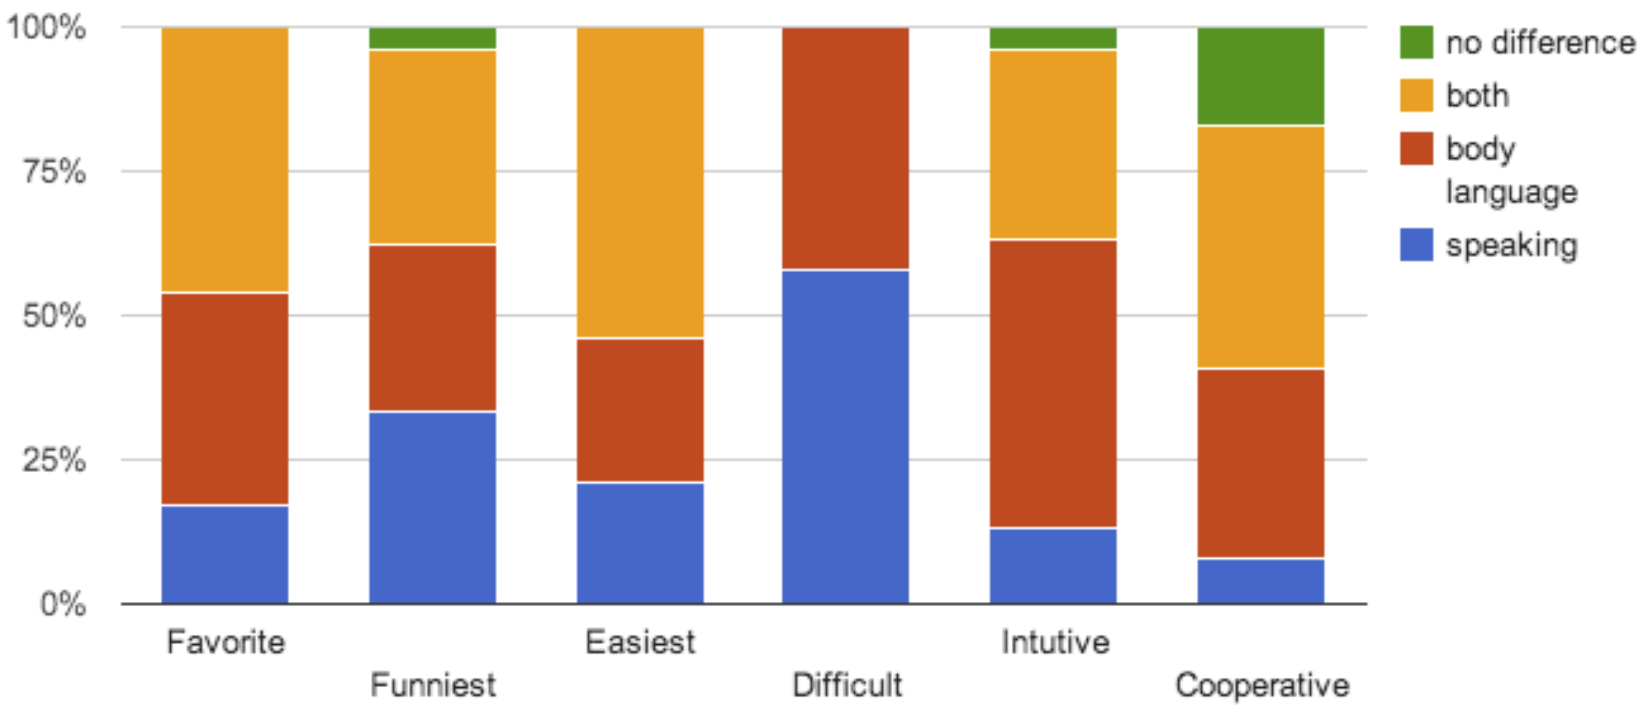
\includegraphics[width=0.9\columnwidth]{Figures/US_FQ_Dif.png}
\caption{Different Language Group}
\label{fig:US_FQ_Dif}
\end{figure}



\subsection{Observation}

\subsubsection{body language consistency}
As we can see in Figure~\ref{fig:US_Consistent} and Table~\ref{tab:Consistency}, we can observe that, with traditional setting (speaking), the eSFQ and CPMs index patterns are inconsistent(the average difference is 22.40\% and 2.90 times). In other words, it's a different game expereience. However, with our body language communication manner design, the eSFQ and CPMs index patterns are similar(the average difference is 6.25\% and 1.00 time). It implies cooperative game has more consistent game experience with body language communication.

\begin{figure}[!h]
\centering
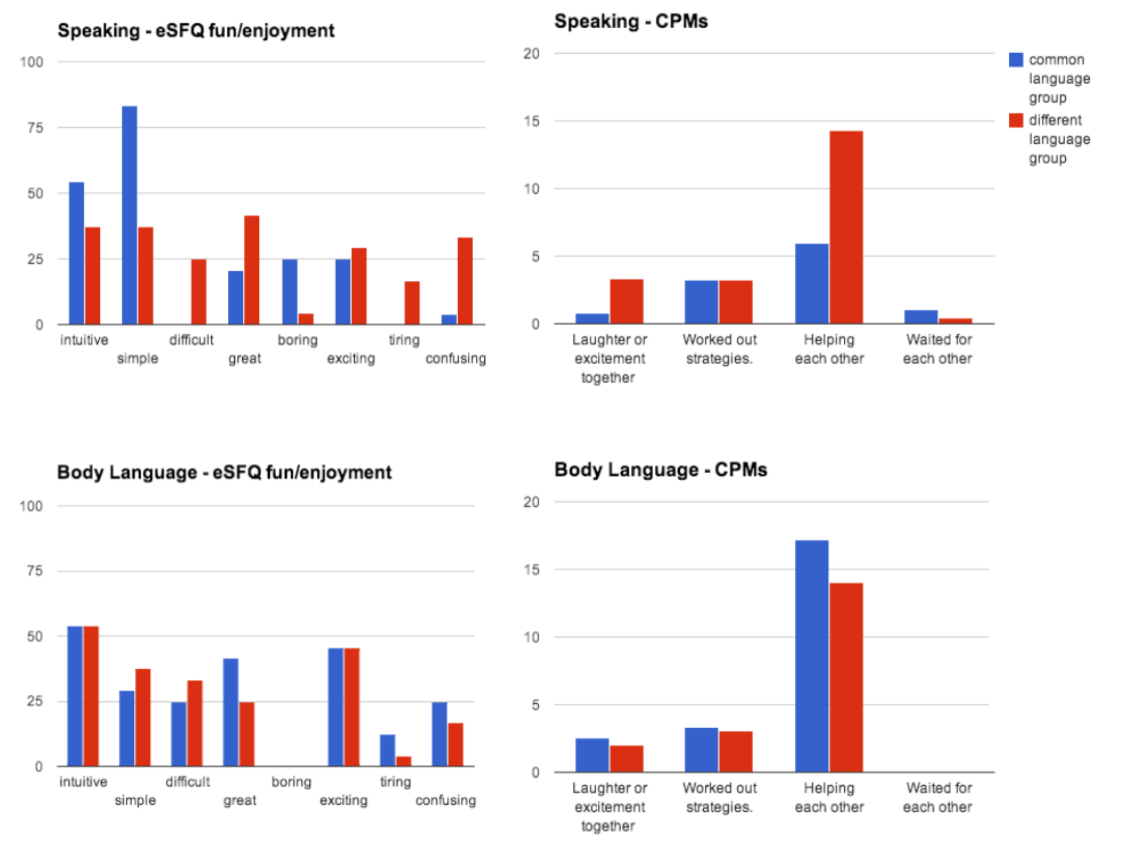
\includegraphics[width=1.1\columnwidth]{Figures/US_Consistent.png}
\caption{index pattern of eSFQ and CPMs}
\label{fig:US_Consistent}
\end{figure}

% \begin{figure}[!h]
% \centering
% \includegraphics[width=0.5\columnwidth]{Figures/US_Consistent2.png}
% \caption{index pattern of CPMs}
% \label{fig:US_Consistent2}
% \end{figure}

\begin{table}[!h]
\renewcommand\arraystretch{1.5}
  \centering
  \begin{tabular}{
  !{\vrule width2pt}c
  !{\vrule width2pt}c
  !{\vrule width2pt}c
  !{\vrule width2pt}}
    \Xhline{2pt}
    \multicolumn{1}
    {!{\vrule width2pt}c!{\vrule width2pt}}
    {\tabhead{}} &
    \multicolumn{1}
    {c!{\vrule width2pt}}
    {\centering\tabhead{eSFQ fun/enjoyment}} &
    \multicolumn{1}
    {c!{\vrule width2pt}}
    {\centering\tabhead{CPMs (count)}} \\
    \Xhline{2pt}
    Speaking & 22.40\% & 2.90  \\
    \Xhline{2pt}
    Body Language & 6.25\% & 1.00 \\
    \Xhline{2pt}
  \end{tabular}
  \caption{Average Difference between common language and different language group from Figure~\ref{fig:US_Consistent}}
  \label{tab:Consistency}
\end{table}


\subsubsection{Communication Pattern}
We want to find out the difference between common language groups and different language group. And we divided them into three section (speaking, body language, and using speaking and body language together) for discussion.

\paragraph{speaking}
When we focus on speaking communication pattern, we compare common language groups and different language groups. We find out that language boundary happened in different langauge groups. However, although there are some language obstacles for different language groups, they still can find some ways as below to communicate with each other.

\begin{enumerate}
  \item Simple is better: users won't choose complicated or tediously long sentences. By contrast, they incline to use simple words to communicate. 
  % For example, such as ``YES'' or ``NO'', use simple words to disassemble complex instruction.

  \item Repeat Continuously: users will use the same words unceasing to express the same meaning until the other user understand.
  
  \item Emphasized tone: users transmit additional information through different tone, such as using brisk tone to express ``everything is allright'' and using urgent tone to express ``something wrong''.
  
  \item Move more: moveing avatar constantly to express some elements such as position, direction etc.
  
  \item Sound simulation: using animal's sound to express animal.
\end{enumerate}

\paragraph{body language}
After our observation, we concluded that there is no difference between common language groups and different language groups when they are using body language to communicate. We integrated all three types of body language communication patterns as below.

\begin{enumerate}
  \item Repeat after me: player who received puzzle-solving hints would perform all the puzzle-solving actions in one go for the other player to observe and emulate. For example, in one of our game stages (see Figure~\ref{fig:US_F2}), the 3 buttons on the floor had to be stepped on one after another in a specific order. The top player would perform the answer all at once for the underside player to repeat. 
 
  \item Step-by-Step: player who received puzzle-solving hints would command the other player to do one action at a time. The next command would not be given until the previous command was executed correctly. For instance, a player jumped in place several times in order to imply that the other player should stand on the object at the corresponding position.
                                  
  \item Pictogram: players would use their own body to express and mimic the hints. As shown in Figure~\ref{fig:US_F3}, one participant wanted to express the letter “N” to the other player. Her solution was using her body to perform pictogram to show the character.
\end{enumerate}

\begin{figure}[!h]
\centering
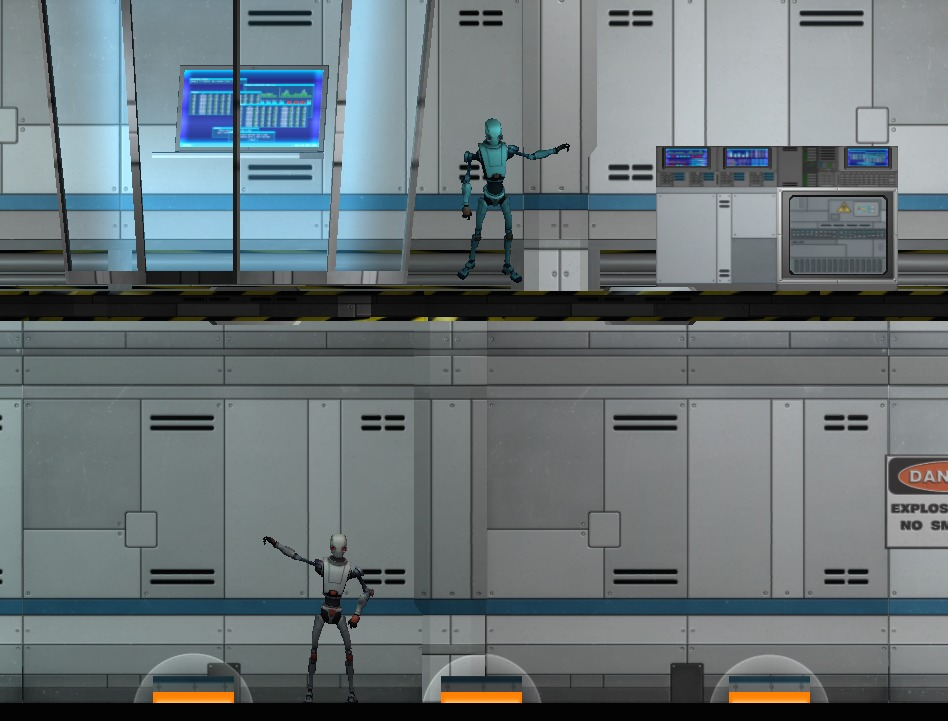
\includegraphics[width=0.7\columnwidth]{Figures/US_F2.jpg}
\caption{A sequence puzzle from Mute Robot. The top player knows the correct sequence and is showing the bottom player to step on the center yellow button among the three buttons.}
\label{fig:US_F2}
\end{figure}

\begin{figure}[!h]
\centering
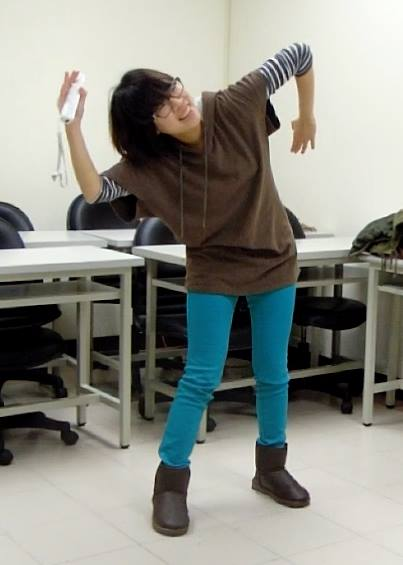
\includegraphics[width=0.4\columnwidth]{Figures/US_F3.jpg}
\caption{A participant performing pictogram (letter “N”) with body language.}
\label{fig:US_F3}
\end{figure}

We also observed that the Step-by-step style is most used across player groups and game stages. In spite of large diversity of body language communication, the players can still find way to communicate effectively.

\paragraph{using speaking and body language together}
In this section, we find out both groups have two communication patterns as below. The difference between groups was the proportion of communication patterns that they used.

\begin{enumerate}
  \item Mixture usage: using both speaking and body language together to transmit messages and assist illustration.

  \item Choosing only one pattern from speaking or body language: users will choose the most suitable or favorite communication manner, and maybe change when special condition happened.
\end{enumerate}


\subsection{Summary}
After our user experiment, user interveiw, questionnaire review and analysis, we integrated some main points for adding body language for cooperative gameplay experience. When we are playing the game, we couldn't understand another player's meaning if there was language obstruction between both of you. In order to relief this perplexity, users needed to guess what each other wanted to express. This means that they need one more language transformation until they build up their tacit agreement. We called this ``Guess Process''. During this process, users will have more interaction with each other such as helping each other. Most of these interaction was interesting to users. And 
% it also increased game difficulty indirectly which 
game enjoyment become higher than before.

\paragraph{1. speaking}
% Now we concluded each section respectively. 
For ``Speaking'', it resulted in enormous difference gameplay experience between common language and different language group. In different language group, player couldn't realize what another player wanted to express and thus they could just guess about another player's meaning under ``Guess Process''. Guess process not only made the enhancement of game difficulty but it also increased game amusement. 
% However cooperative feeling and curiosity won't increase. 

\paragraph{2. body language}
% In addition, 
About ``body language'', Both common language and different language group would occur ``Guess Process'', which increased gameplay enjoyment for both group. Body language provided great cooperative experience.
% and enhanced players' curiosity significantly to the game. 
In this section, gameplay difficulty was similar to all players, which meaned it had difficulty normalization and applied identically gameplay experience.

\paragraph{3. using speaking and body lanuguage together}
% Last but not least, 
About section of ``using speaking and body language together'', was the condition that add the ``body language'' element on the basic of ``speaking''. Although language obstacle had an impact on gameplay experience no matter on common language group or different language group, the enjoyment of playing the game were better than traditional manner (speaking). 
% Cooperative feeling and curiosity also increased obviously. Even more interesting is that under this section, different language group are the easiest and also the most interesting manner to communicate. For this result, we thought it was because the cooperative experience had greater influence on gameplay enjoyment than the difficulty.



